\documentclass{beamer}

\mode<presentation>
{
  \usetheme{CambridgeUS}
  \setbeamercovered{invisible}
}

\usepackage[english]{babel}
\usepackage[latin1]{inputenc}
\usepackage{times}
\usepackage[T1]{fontenc} 
% Or whatever. Note that the encoding and the font should match. If T1
% does not look nice, try deleting the line with the fontenc.
\usepackage{amsmath}

\newcommand{\linespace}{\vskip 0.25cm}

% The text in square brackets is the short version of your title and will be used in the
% header/footer depending on your theme.
\title{A detailed analysis of a PushGP run}
%{Using Graph Databases to Explore Genetic Programming Run Dynamics}

% Sub-titles are optional - uncomment and edit the next line if you want one.
\subtitle{Rooting through the relics of digital evolution} 

% The text in square brackets is the short version of your name(s) and will be used in the
% header/footer depending on your theme.
\author[Nic McPhee]{Nic McPhee (w/ Finzel, Casale, Helmuth, \& Spector)}

% The text in square brackets is the short version of your institution and will be used in the
% header/footer depending on your theme.
\institute[UMN Morris]
{
  Division of Science and Mathematics \\
  University of Minnesota, Morris \\
  Morris, Minnesota, USA \\
}

% The text in square brackets is the short version of the date if you need that.
\date[May 2016, GPTP, Ann Arbor MI] % (optional)
{May 2016 \\ Genetic Programming Theory and Practice \\ University of Michigan \\ Ann Arbor, MI}

% Delete this, if you do not want the table of contents to pop up at
% the beginning of each subsection:
\AtBeginSection[]
{
  \begin{frame}<beamer>
    \frametitle{Outline}
    \tableofcontents[currentsection, hideothersubsections]
  \end{frame}
}

\begin{document}

\begin{frame}
  \titlepage
\end{frame}

% For a 20-25 minute senior seminar talk you probably want something like:
% - Two or three major sections (other than the summary).
% - At *most* three subsections per section.
% - Talk about 30s to 2min per frame. So there should probably be between
%   15 and 30 frames, all told.

\section*{Overview}

\subsection*{The Big Picture}

\begin{frame}
  \frametitle{The Big Picture}
  
  \begin{itemize}
	\item Genetic programming clearly \emph{works}.
	\item But we rarely know \emph{why} or \emph{how}.
	\item Databases allow examination of the internal interactions of a run.
	\item Graph databases allow us to collect and analyze lineages.
	\item Silico-paleontology can help us understand and improve our tools.
  \end{itemize}

\end{frame}

\subsection*{Outline}

\begin{frame}
  \frametitle{Outline}
  \tableofcontents[hideallsubsections]
\end{frame}

\section{What do we know? (And how do we talk about it?)}

\subsection{We throw so much away}

\begin{frame}{We keep/see/share so little}
			EC research has the potential to generate \emph{huge} amounts of data.
			\linespace
			What do we normally do with that data?
			\linespace
			We typically throw it away -- \& paleontologists weep!
			\linespace
			\centering
			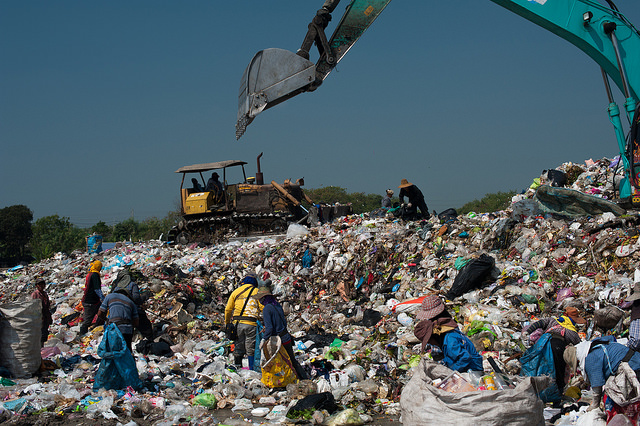
\includegraphics[width = 0.6 \linewidth]{../../figures/Harvest.jpg} \\
			\tiny{\url{https://www.flickr.com/photos/thibaud_saintin/12533059215/}}
			% \textbf{Get bulldozer on dump photo}
\end{frame}

\subsection{Let's go hunting for beetles!}

\begin{frame}{Let's trade the forest for the trees}
	We typically share summary results (tables, graphs) that represent a 30,000 foot view of (part of) the forest.
	\linespace
	We'll instead focus on a single tree, in places peeling back the bark and poking at the beetles we find underneath.
	\linespace
	\linespace
	This is not a ``one or the other'' question. There is important value in understanding
	the behavior of large-scale ecosystems, as well as understanding the details of
	organisms in those ecosystems.
\end{frame}

\section{Tools, problem, and setup}

\begin{frame}{PushGP/Clojush}
	\begin{itemize}
		\item PushGP: Stack-based GP system; multiple types; successful in a variety of domains
		\item Plush genomes: More in Lee's talk; linear representation that maps to structured Push programs.
		\item Operators: Alternation (form of n-point crossover with shifts), ``point'' mutation, and \emph{close} mutation
		\item Lexicase selection: Avoid aggregation; shuffle test cases afresh for each selection and select lexicographically using that ordering
		\item Population size = 1,000
	\end{itemize}
	The example here uses PushGP, etc., but could be applied to most any evolutionary system.
\end{frame}

\begin{frame}{Replace-space-with-newline problem}
	Replace-space-with-newline is from software synthesis benchmark suite that was central to Tom Helmuth's dissertation last year.
	\begin{itemize}
		\item Two related goals. Given an input string:
		\begin{itemize}
			\item \emph{Print} the string with all the spaces replaced by newlines.
			\item \emph{Return} (on the \texttt{integer} stack) the number of \emph{non-space} characters in the input string.
		\end{itemize}
		\item Error vector with 200 values, one for each type of error across 100 test cases
	\end{itemize}
	
	This problem has a roughly 50\% success rate with described setup.
	\linespace
	We'll focus on a run that succeeded quickly (30 generations)
\end{frame}

\begin{frame}{DB \& visualization tools}
	Graph database tools:
	\begin{itemize}
		\item Titan graph database (an Apache project)
		\item Tinkerpop graph query language
		\item Gremlin shell
	\end{itemize}
	\linespace
	Graph visualizations created with Graphviz.
\end{frame}

\section{Visualizing ancestries}

\subsection{Full ancestry graphs}

\begin{frame}{Full ancestry of ``winners''}
	\centering
	\includegraphics[width=\linewidth]{../../figures/run0_GPTP_2_font_40}
\end{frame}

\begin{frame}{Full ancestry of ``winners'' (sized and colored)}
		\begin{overprint}
		\onslide<1-3> 			\centering
		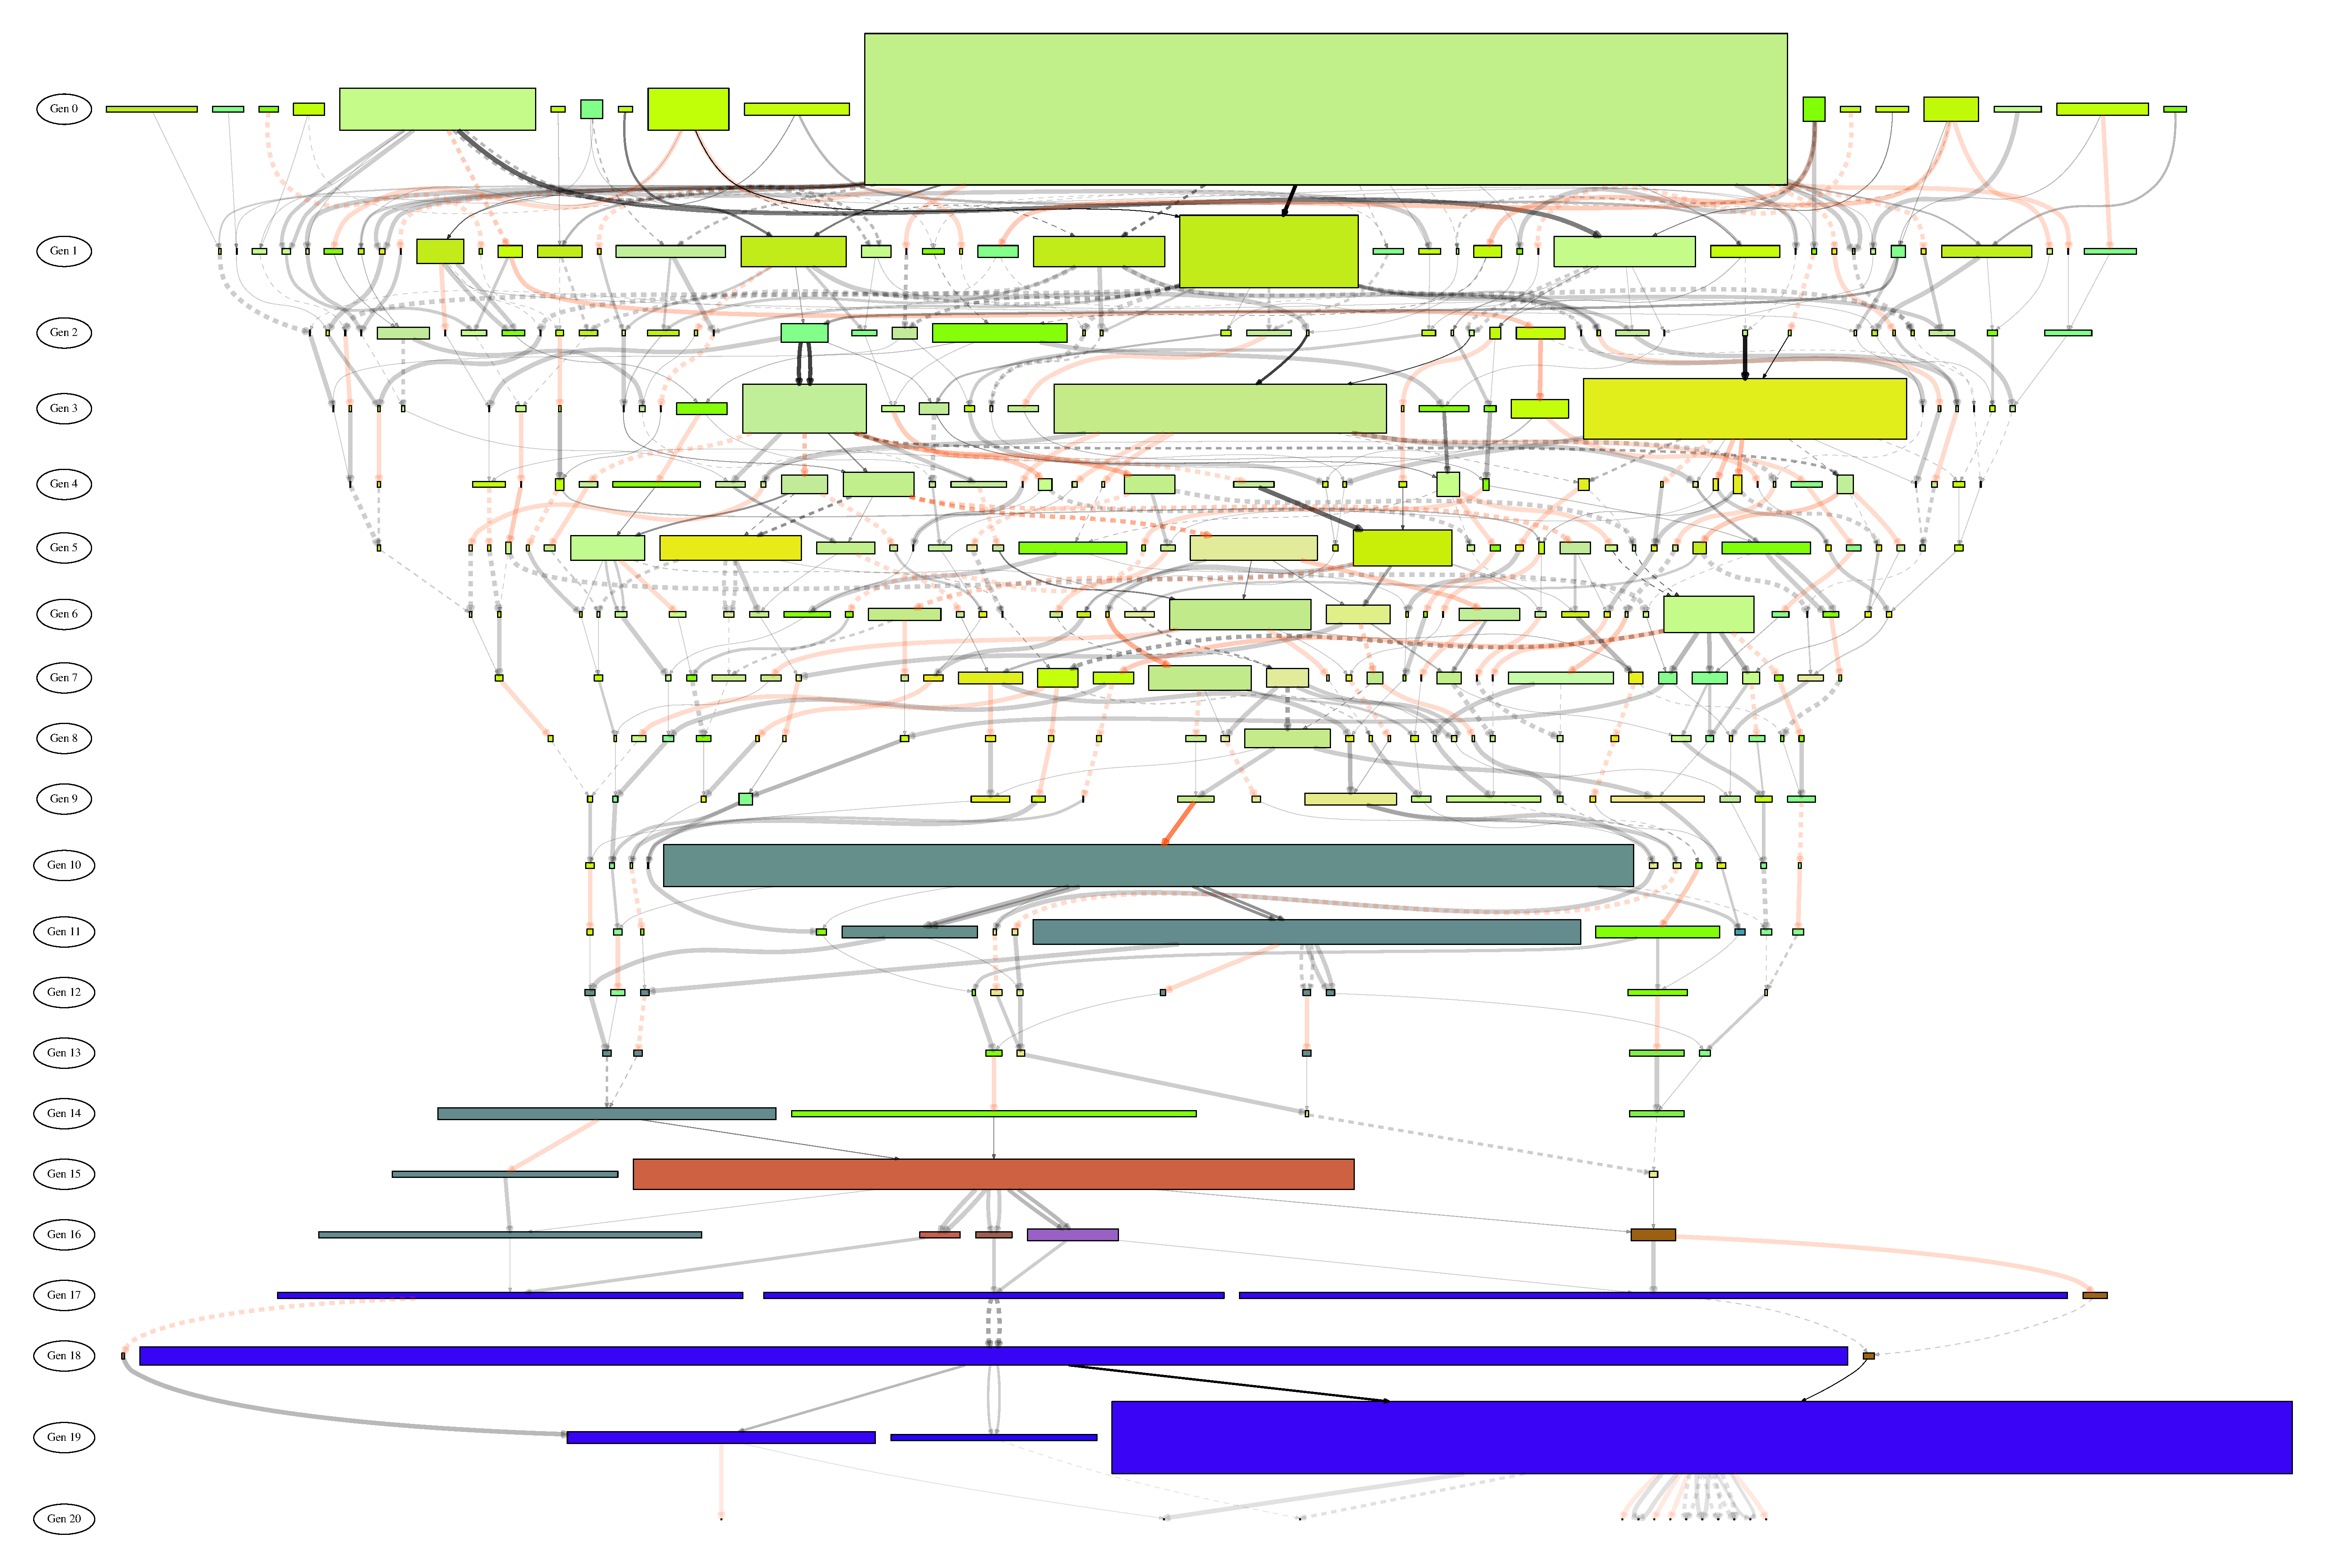
\includegraphics[width=0.7\linewidth]{../../figures/run0_RBM_color_full_30000}
		\onslide<4> 			\centering
		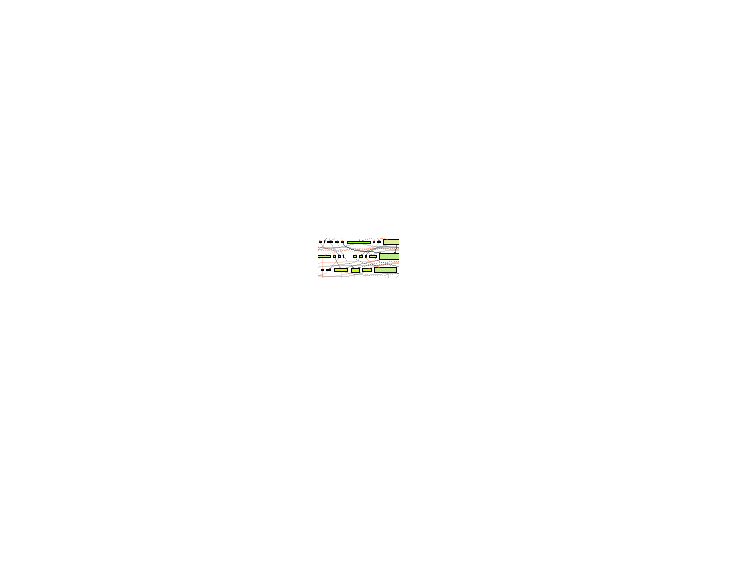
\includegraphics[width=0.9\linewidth]{../../figures/run0_colored_detail}
		\end{overprint}
	\begin{overprint}
		\onslide<1>
		Width of boxes is proportional to number of selections
		\onslide<2>
		Heights are proportional to number of children \emph{in this graph}
		\onslide<3>
		Colors are a compression of the \emph{error vectors} (200 errors to RGB colors)
		\onslide<4>
		Edges encode genetic ops and level of genetic contribution of parents
	\end{overprint}
\end{frame}

\subsection{Filtering ancestries}

\begin{frame}{Why we want to filter ancestries}
	\begin{center}
	\includegraphics[width=\linewidth]{../../figures/run0_GPTP_2_font_40}
	\end{center}
	\linespace
	Busy and dense, even for a very short run like this
\end{frame}

\begin{frame}{Why we want to filter ancestries}
	\begin{columns}
		\begin{column}{0.4 \linewidth}
			Vastly worse for longer runs like this! (129 generations)
			\linespace
			And we have much bigger data sets than this, with thousands of generations
			\linespace
			So let's try to filter the ancestries to focus on the individuals ``that matter''.
		\end{column}
		\begin{column}{0.6 \linewidth}
\begin{center}
	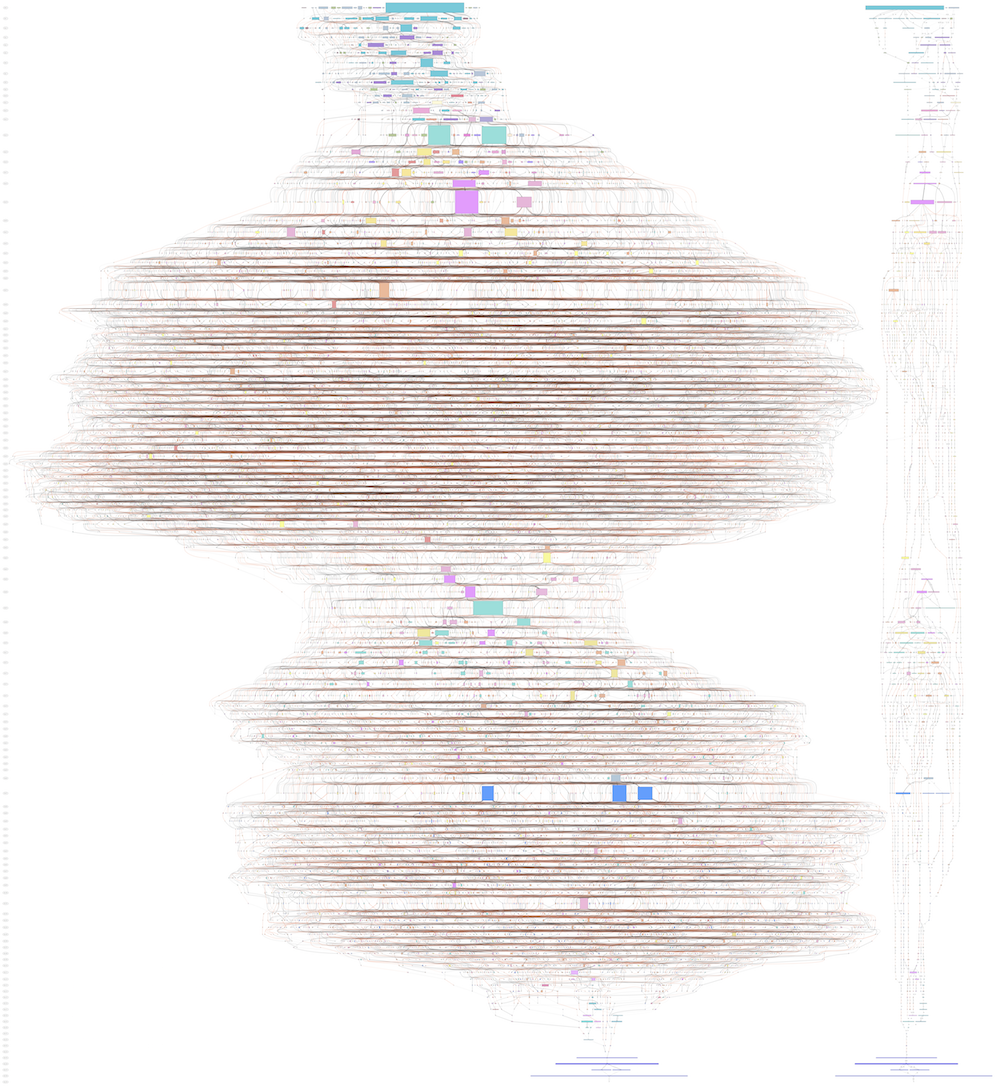
\includegraphics[height=0.8\textheight]{../../figures/run1_RBM_color_filtered_and_full_60000.png}
\end{center}
\end{column}			
	\end{columns}
\end{frame}

\begin{frame}{A simplistic approach to filtering}
	We want to focus on the individuals that contributed the most to their offspring.
	\linespace
	Compute the Damerau-Levenshtein distance between parent-child genomes and eliminate ``far'' parent if:
	\begin{itemize}
		\item The ``near'' parent is \emph{very} near (so it contributes all or almost all the genetic material)
		\item The ``far'' parent is at least twice as far as the ``near'' parent
	\end{itemize}
	These are really a simplistic hack to let us quickly focus on what are \emph{likely} to be the most important parts of the graph, but they can oversimplify (as we'll see later).
\end{frame}

\begin{frame}{Filtered version of our target run}
	\begin{center}
		
\includegraphics[width=\linewidth]{../../figures/run0_RBM_color_filtered_and_full_30000}
	\end{center}
\end{frame}

\section{Exploring a run in detail}

\begin{frame}{Exploring a run in detail}
	
	\begin{columns}
		\begin{column}{0.55 \linewidth}
			\centering
			%\includegraphics[width = \linewidth]{Figures/run6_lexicase_rswn_diversity.pdf}
		\end{column}
		
		\begin{column}{0.4 \linewidth}
			\begin{overprint}
				\onslide<1>
				Focusing on one successful L run now.
				\linespace
				Three big diversity changes:
				\begin{itemize}
					\item First 15 generations have a sharp drop then steep rise
					\item Around generation 40 a sharp drop and rise
					\item Sharp drop at end just before a solution is found
				\end{itemize}
				
				\onslide<2>
				\emph{What's happening at those sections of the run?}
				\linespace
				We want to be able to dig through a run and see what happened.
			\end{overprint}
		\end{column}
	\end{columns}
\end{frame}

\section[Using a graph DB]{Using a graph database}

\subsection{Goals}

\begin{frame}{Goals}
	\begin{columns}
		\begin{column}{0.6 \linewidth}
					We want to store and analyze \emph{all} the individuals and their relationships.
					\linespace
					Ancestry relationships are naturally modeled with a graph
					\linespace
					So graph databases seem a natural tool for the relationship part.
					\linespace
					\centering
					%\includegraphics[width=0.8 \linewidth]{Figures/olemartin_family_tree.jpg} \\
					\tiny{\url{www.hokstad.com/family-tree-using-graphviz-and-ruby}}
		\end{column}
		\begin{column}{0.4 \linewidth}
			%\includegraphics[height= 0.75 \textheight]{Figures/HeuristicLabGraph.pdf} \\
			\tiny{\cite{Burlacu:2013:VGL:2464576.2482714}}
		\end{column}		
	\end{columns}
\end{frame}

\subsection{Neo4j}

\begin{frame}{Neo4j graph database}
	
\begin{columns} 
\begin{column}{0.65 \textwidth}
		\begin{itemize}
			\item Part of the new-ish NoSQL movement
			\begin{itemize}
				\item Neo4j's initial release was 2007
				\item Started to take off in 2010
			\end{itemize}
			\linespace
			\item Represent individuals as nodes
			\item Represent parent-child relationships as edges
			\linespace
			\item Easy to represent complex relationships
			\item Easy to \emph{search} for relationships
			\item Efficient recursive queries, esp. compared to traditional databases
		\end{itemize}
		\end{column}
		\begin{column}{0.35\textwidth}
			\centering
	   %\includegraphics[width=0.95\textwidth]{Figures/graphdb-neo4j.png}
       \\
    \tiny{\url{http://neo4j.com}}
  \end{column}
  \end{columns}

\end{frame}

\subsection{Cypher}

\begin{frame}{Cypher query language}
			Neo4j uses the \emph{Cypher} query language.
			
			\linespace
			
			~\\
			
			\linespace

	\begin{columns}
		\begin{column}[T]{0.5\textwidth}
			
			Fundamental elements of Cypher queries:
		\begin{itemize}
			\item START
			\item MATCH
			\item WHERE
			\item RETURN
		\end{itemize}
		
	\end{column}
	\begin{column}[T]{0.5\textwidth}
		Uses "ASCII art" to describe relationships:
	
	\linespace
\begin{center}
	(p)-$\,$->(c) \\
	\linespace
	(p)-[r:PARENT\_OF]->(c)
\end{center}

	\end{column}	
	\end{columns}
\end{frame}

\begin{frame}{Can model (complex) paths}
	Find Nic's parents:
	
	\begin{center}
		\texttt{(Nic)<-[:PARENT\_OF]-(p)}
	\end{center}

	Find all Nic's grandparents:
	
	\begin{center}
		\texttt{(Nic)<-[:PARENT\_OF*2]-(gp)}
	\end{center}
	
		Find everyone at most 5 steps from Nic:
		
		\begin{center}
			\texttt{(Nic)<-[:PARENT\_OF*1..5]-(a)}
		\end{center}
		
	Find all Nic's siblings:
	
	\begin{center}
		\texttt{(Nic)<-[:PARENT\_OF]-()-[:PARENT\_OF]->(s)}
	\end{center}
	
\end{frame}

\section{Let's go exploring!}

\subsection{Setup}

\begin{frame}{What are we exploring?}
Tom Helmuth provided a \emph{lot} of data:
\begin{itemize}
	\item A number of program synthesis problems taken from intro computing texts
	\item Three different selection mechanisms: Lexicase, tournament, and implicit fitness sharing (IFS)
	\item All using Clojush implementation of Lee Spector's PushGP system \url{https://github.com/lspector/Clojush}
	\item Population size 1,000; $\leq 300$ generations
\end{itemize}
See \cite{Helmuth:GECCO15} for more.

\linespace

We used \texttt{batch-import} tool and custom scripts to import into Neo4j. 
{\tiny \url{https://github.com/jexp/batch-import}} 
\end{frame}

\begin{frame}{Only just the beginning}
	\begin{itemize}
		\item We have data from hundreds of runs
		\item Currently a very ``by hand'' process
		\item Definitely learned valuable things about:
		\begin{itemize}
			\item The behavior of lexicase
			\item Role of alternation (a type of crossover) in PushGP
			\item Impact of test cases on evolutionary dynamics
		\end{itemize}
	\end{itemize}
	
	\linespace
	
	We'll look at results from two runs:
	\begin{itemize}
		\item Both successful on replace-space-with-newline problem
		\item One using lexicase (sol'n found in 88 gens)
		\item One using tournament selection (sol'n found in 151 gens)
	\end{itemize}
\end{frame}

\subsection{Comparing the end-games}

\begin{frame}{How did we construct a winner?}
	How is a winner constructed at the end of a run?
	
	\linespace
	
	This query finds all ancestors of a winner (zero \texttt{total\_error}) going back at most 8 steps:
	
	\linespace
	
	\texttt{$\quad$ MATCH (w) WHERE w.total\_error = 0 \\ % \{total\_error: 0\}) \\
		% $\quad$ WHERE w.total\_error = 0 \\
		$\quad$ MATCH (p)-$\,$->(c)-[*0..7]->(w) \\
$\quad$ RETURN DISTINCT id(p), id(c);}

	\linespace
	
	8 steps is fairly arbitrary; returns a small enough set to visualize.
\end{frame}

\begin{frame}{Comparing the end-games}
	\begin{columns}
		\begin{column}{0.5 \linewidth}
			Ancestry of winner(s) look very different
			\begin{itemize}
				\item Tournament selection (below): Single winner w/ high branching factor
				\item Lexicase (right): 45 winners w/ much lower branching factor
			\end{itemize}
			\begin{center}
				%\includegraphics[width=\linewidth]{Figures/ancestors_of_winner_rswn_tourney_run74_9gens}
			\end{center}
		\end{column}
		\begin{column}{0.5 \linewidth}
			\begin{center}
				%\includegraphics[width=\linewidth]{Figures/ancestors_of_winners_colons}
			\end{center}
		\end{column}
	\end{columns}
\end{frame}

\begin{frame}{Lexicase selection}
	\begin{columns}
		\begin{column}{0.5 \linewidth}
			%\includegraphics[height=0.9\textheight]{Figures/ancestors_of_winners_colons}
		\end{column}
		\begin{column}{0.45 \linewidth}
			\begin{overprint}
				\onslide<1>
			A number of observations:
			\begin{itemize}
				\item 45(!) ``winning'' individuals
				\item Individual ``86:261'' is (a) parent of all 45
				\item Individual ``86:261'' is a parent of 934 (of 1,000) individuals in next generation
			\end{itemize}
			
			\onslide<2>
			Seriously?!? 934 offspring?!?
			
			\linespace
			
			Turns out to an be extreme case of a common phenomena with lexicase
			
			\linespace
			
			Nodes marked with diamonds all had at least 100 offspring
			
			\linespace
			
			Shaded diamonds also have at least 5 offspring that are ancestors of or are winners
			
			\onslide<3-4>
			What's the total error (fitness) of ``86:261''?
			\begin{itemize}
				\item<4> 4,034(!)
				\item<4> Bottom quartile!
				\item<4> But had 934 offspring! \linespace
				\item<4> Failed to return on 4 cases (error 1,000 each)
				\item<4> Got 2 other answers wrong (error 17 each)
				\item<4> Terrible total error, but perfect on 194 of 200 tests
				\item<4> Great for lexicase!
			\end{itemize}
						
			\onslide<5-6>
			What's the total error (fitness) of ``85:086''?
			\begin{itemize}
				\item<6> \emph{100,000!}
				\item<6> Rank 971 out of 1,000
				\item<6> But had 180 offspring \linespace
				\item<6> Got all the ``print'' cases
				\item<6> Failed to return value for all 100 ``return'' cases (error 1,000 each)
				\item<6> \emph{Terrible} total error, but perfect on 100 of 200 tests
				\item<6> Fine for lexicase
			\end{itemize}
			
			\onslide<7>
			High proportion of mutations:
			\begin{itemize}
				\item Roughly half the offspring in this graph created via mutation
				\item Probably why there's less branching
			\end{itemize}
			
			\end{overprint}
		\end{column}
	\end{columns}
\end{frame}

\begin{frame}{Tournament selection}
	%\includegraphics[width=\linewidth]{Figures/ancestors_of_winner_rswn_tourney_run74_9gens}
	\vspace{-1cm}
	\begin{itemize}
		\item Much broader: 42 ancestors of a winner for tournament 9 gens back; 14 for lexicase
		\item About two-thirds created via crossover, so more branching than lexicase
	\end{itemize}
\end{frame}

\begin{frame}{Number ancestors of ``winners'' over time}
		\begin{center}
			\begin{tabular}{rrr}
				Gens from winner & Lexicase & Tournament \\
				\hline\noalign{\smallskip}                
                1 & 4 & 2 \\
                2 & 6 & 4 \\
                3 & 7 & 6 \\
                4 & 6 & 10 \\
                5 & 7 & 13 \\
                6 & 9 & 20 \\
                7 & 10 & 30 \\
                8 & 14 & 33 \\
                9 & 14 & 42 \\
                10 & 22 & 63 \\ 
%                \ldots \\
%                15 & 49 & 152 \\
                \vdots & \vdots & \vdots \\ 
                18 & 58 & 297 \\
			\end{tabular}
		\end{center}
\end{frame}

\begin{frame}{12 most fecund individuals}
		\begin{center}
			\begin{tabular}{rr}
				Lexicase & Tournament \\
				\hline\noalign{\smallskip}
				934 & 24 \\
				657 & 23 \\
				594 & 23 \\
				590 & 21 \\
				433 & 20 \\
				326 & 20 \\
				297 & 19 \\
				294 & 19 \\
				285 & 19 \\
				283 & 18 \\
				279 & 18 \\
				271 & 18 \\
			\end{tabular}
		\end{center}
\end{frame}

\section[Conclusions]{Conclusions}

\begin{frame}
\frametitle{Conclusions}

Still early days, but we can definitely see some useful things:
\begin{itemize}
\item Differences in ways selection mechanisms work
\item Support for hypotheses (e.g., Tom's paper)
\item Evidence for importance of crossover in PushGP
\item Impact of test cases on evolutionary dynamics
\end{itemize}

\linespace
\linespace

Future Work
\begin{itemize}
\item Automate more of the work
\item Examine more runs/problems/etc.
\item Explore how to include this ``on-line''
\end{itemize}
\end{frame}

\begin{frame}{Thanks!}
	
	Thank you for your time and attention!

	\linespace
	
	Thanks to M. Kirbie Dramdahl (University of Minnesota, Morris), and to Lee Spector's Computational Intelligence group (Hampshire College) for ideas and feedback.
	
	\linespace
	
	Contacts:  
	\begin{itemize}
		\item \texttt{mcphee@morris.umn.edu}
		\item \texttt{donat056@morris.umn.edu}
		\item \texttt{thelmuth@cs.umass.edu}
	\end{itemize}
	
	\linespace
	\linespace
	
	\begin{center}
	{\huge Questions?}
	\end{center}
\end{frame}

\section*{References}

\begin{frame} 
\frametitle{References}
\bibliographystyle{apalike}
{\tiny \bibliography{GraphDBandGP}}
\end{frame} 

\end{document}


